\documentclass[../template]{subfiles}

\begin{document}
\section{Shortest Path}
\subsection{Algoritmo di Dijkstra}
Applicabile soltanto nel caso in cui i pesi degli archi siano sempre non negativi.

\begin{center}
    \begin{tikzpicture}[rotate=90]
        \Vertices[unit=2.1]{circle}{0, 1, 2, 3}
        \tikzset{EdgeStyle/.style={->, bend right=18}}
        \Edge[label=$3$, color=red](0)(1)
        \Edge[label=$12$](0)(2)
        \Edge[label=$16$](0)(3)
        \Edge[label=$9$](1)(0)
        \Edge[label=$18$](1)(2)
        \Edge[label=$7$, color=red](1)(3)
        \Edge[label=$5$](2)(0)
        \Edge[label=$3$, color=red](2)(3)
        \Edge[label=$8$](3)(0)
        \Edge[label=$1$](3)(2)
        ;
    \end{tikzpicture}
\end{center}
\lstinputlisting{algorithms/dijkstra.py}
\subsubsection{Dimostrazione Correttezza}
%48m lezione 5
La dimostrazione viene effettuata per ragionamento induttivo sui due seguenti punti:
\begin{enumerate}
    \item $\forall y \in V$, il valore \lstinline{dist[y]} rappresenta ad ogni iterazione la lunghezza
        del cammino minimo da \lstinline{source} a \lstinline{y}, passando solo attraverso i nodi contenuti in  $W$.
        \lstinline{dist[y] == None} indica che il nodo non è raggiungibile passando solamente attraverso i nodi di $W$.
        In \lstinline{parent[y]} è memorizzato il nodo che precede immediatamente $y$ in tale cammino.
        \lstinline{parent[source] == None} indica che \lstinline{source} non è preceduto da altri nodi.

    \item quando il nodo $x$ viene aggiunto a $W$, il valore \lstinline{dist[x]} rappresenta la distanza minima tra
        \lstinline{source} e $x$.  Il cammino minimo è ricostruibile procedendo a ritroso partendo da \lstinline{parent[x]}.
\end{enumerate}
Per $n = i = 0$ sono ovviamente vere entrambe.

\subsubsection{Dimostrazione punto 1}
Per il passo $n = i+1$, quando analizziamo $y$, abbiamo due casi possibili:
$x$ non è contenuto all'interno del cammino minimo, per cui, per ipotesi induttiva, la distanza minima è \lstinline{dist[y]};
oppure $x$ precede immediatamente $y$ nel cammino minimo, quindi in tal caso deve avere distanza \lstinline{dist[x] + weight[x][y]}.

% 1h:03
Consideriamo per assurdo che $x$ non preceda immediatamente $y$, allora $\exists t \in W$ nel cammino minimo tra $x$ ed $y$,
il cammino da $s$ a $t$, per ipotesi induttiva, ha almeno una lunghezza che è $\ge$ \lstinline{dist[t]}, con relativo cammino minimo
che non comprende $x$.
Il cammino da \lstinline{source} a $y$, passante per $x$ è quindi sostituibile da un' altro cammino di lunghezza inferiore, non passante
per $x$, ma questo ricadrebbe nel primo caso, dove $x$ non è contenuto all'interno del cammino minimo.

\subsubsection{Dimostrazione punto 2}
per assurdo, ipotizziamo che esista un cammino da $s$ a $x$ di lunghezza inferiore a $\rho(x)$ che passi per nodi $\notin W$, chiamato $z$
il primo di tali nodi.
Chiamato $L(s, x)$, la lunghezza del cammino passante per $z$, abbiamo che per ipotesi per assurdo: $L(s, z) + L(z, x) < \rho(x)$.
Osserviamo che $L(s, z) \ge \rho(z)$ perché tra $s$ e $z$ tutti i nodi sono contenuti in $W$, e $\rho(z)$ è la lunghezza minima
dei cammini da $s$ a $z$ non passanti per nodi al di fuori di $W$.
$L(z, x) \ge 0$ perché per ipotesi tutte le distanze sono non negative, quindi abbiamo:
\[
    \rho(z) \le L(s, z) + L(z, x) = L(s, x) < \rho(x)
\]
Siamo giunti ad un assurdo perché, da come è definito l'algoritmo $x = \arg\min\limits_{y\notin W}\{\rho(y)\}$, e di
conseguenza $\rho(x) < \rho(z)$.
\subsubsection{Complessità}
Il numero di operazioni richiesto è $O(V^2)$, dovuta ad il ciclo principale di complessità $O(|V|)$ ed il
calcolo del minimo ed il ciclo sui nodi adiacenti, entrambi di complessità $O(|V|)$.

\newpage
\subsection{Operazione di Triangolazione}
Data una matrice $n \times n$ di distanze $R$, per un dato $j \in \{1\ldots n\}$, chiamiamo ``operazione di triangolazione'' il
seguente aggiornamento:
\[
    R_{jk} = \min\big\{R_{ik}, R_{ij} + R_{jk}\big\} \quad \forall\,i, k \in \big\{1\ldots n\big\} - \big\{j\big\}
\]
\subsection{Algoritmo di Floyd-Warshall}
Applicabile solo se nel grafo non sono presenti cicli di lunghezza negativa. Restituisce la lunghezza dei cammini minimi tra ogni
coppia di nodi.
\lstinputlisting{algorithms/floyd_warshall.py}

\subsubsection{Note}
In caso di distanze $d_{ij} > 0$, la condizione di arresto $R_{ij} < 0$ non si potrà mai verificare, e si dimostra che i valori di
$R_{ij}$ danno la lunghezza del cammino minimo da $i$ a $j$ per ogni $i \neq j$, mentre le etichette $E_{ij}$ consentono di ricostruire tali
cammini minimi.

In caso di distanze negative, se non interviene la condizione di arresto $R_{ii} < 0$, allora anche qui gli $R_{ij}$ danno la lunghezza del
cammino minimo da $i$ a $j$.

Se invece ad una certa iterazione si verifica la condizione $R_{ii} < 0$, indica la presenza di un ciclo a costo negativo nel grafo. In tal caso,
anche ignorando la condizione di arresto $R_{ii} < 0$, non possiamo garantire che al memento della terminazione con $j = n$ gli $R_{ij}$ diano la lunghezza del cammino minimo da $i$ a $j$.

\subsubsection{Complessità}
È facile osservare che la complessità per questo algoritmo è $O(|V|^3)$, dovuta ai tre cicli nidificati, ognuno di complessità $O(|V|)$.
\subsection{Note}
Entrambi quest algoritmi, rientrano nella categoria di raffinamento locale. Infatti in entrambi i casi, data una coppia di nodi, si
parte da una soluzione ammissibile, e ad ogni iterazione, tale cammino viene aggiornato nel caso se ne trovi uno di lunghezza inferiore.

\end{document}
